\begin{figure*}[t]
\begin{center}
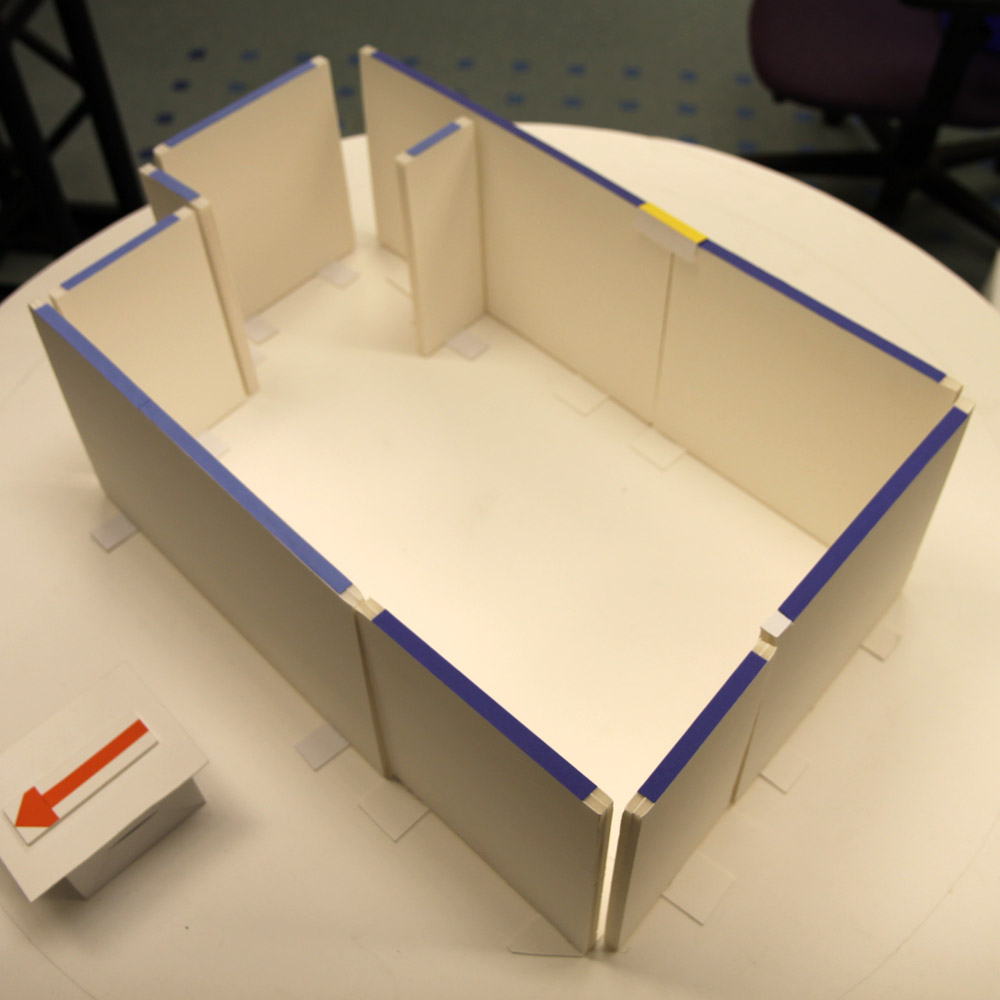
\includegraphics[width=1.9in]{../gi2012_userstudy/images/photos/63_original} %N1
\begin{minipage}[b]{4.9in}
  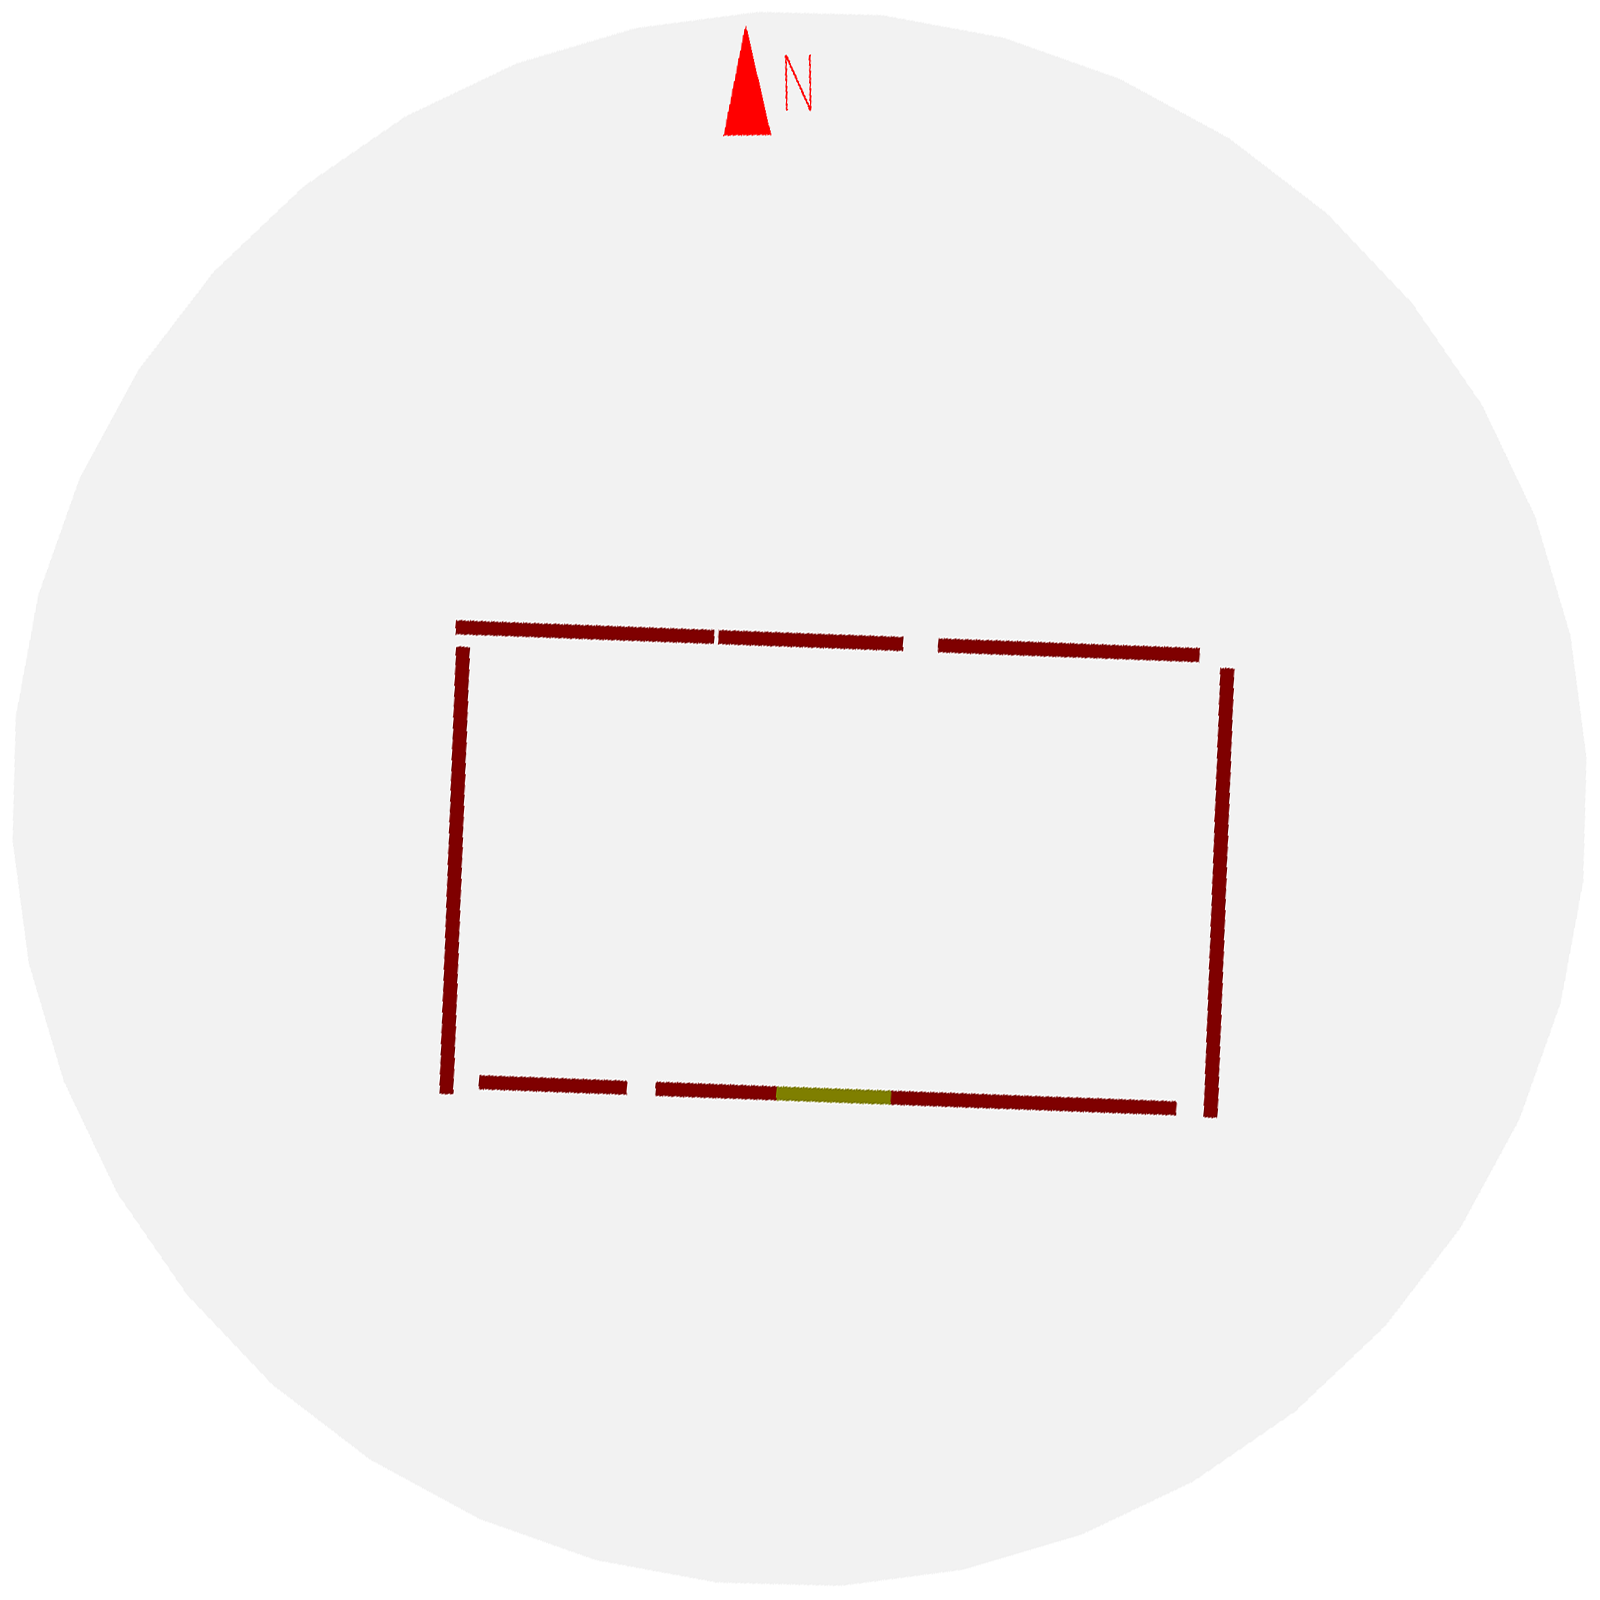
\includegraphics[width=0.95in]{../gi2012_userstudy/images/section2/0_2D_walls_rotate} %A1
  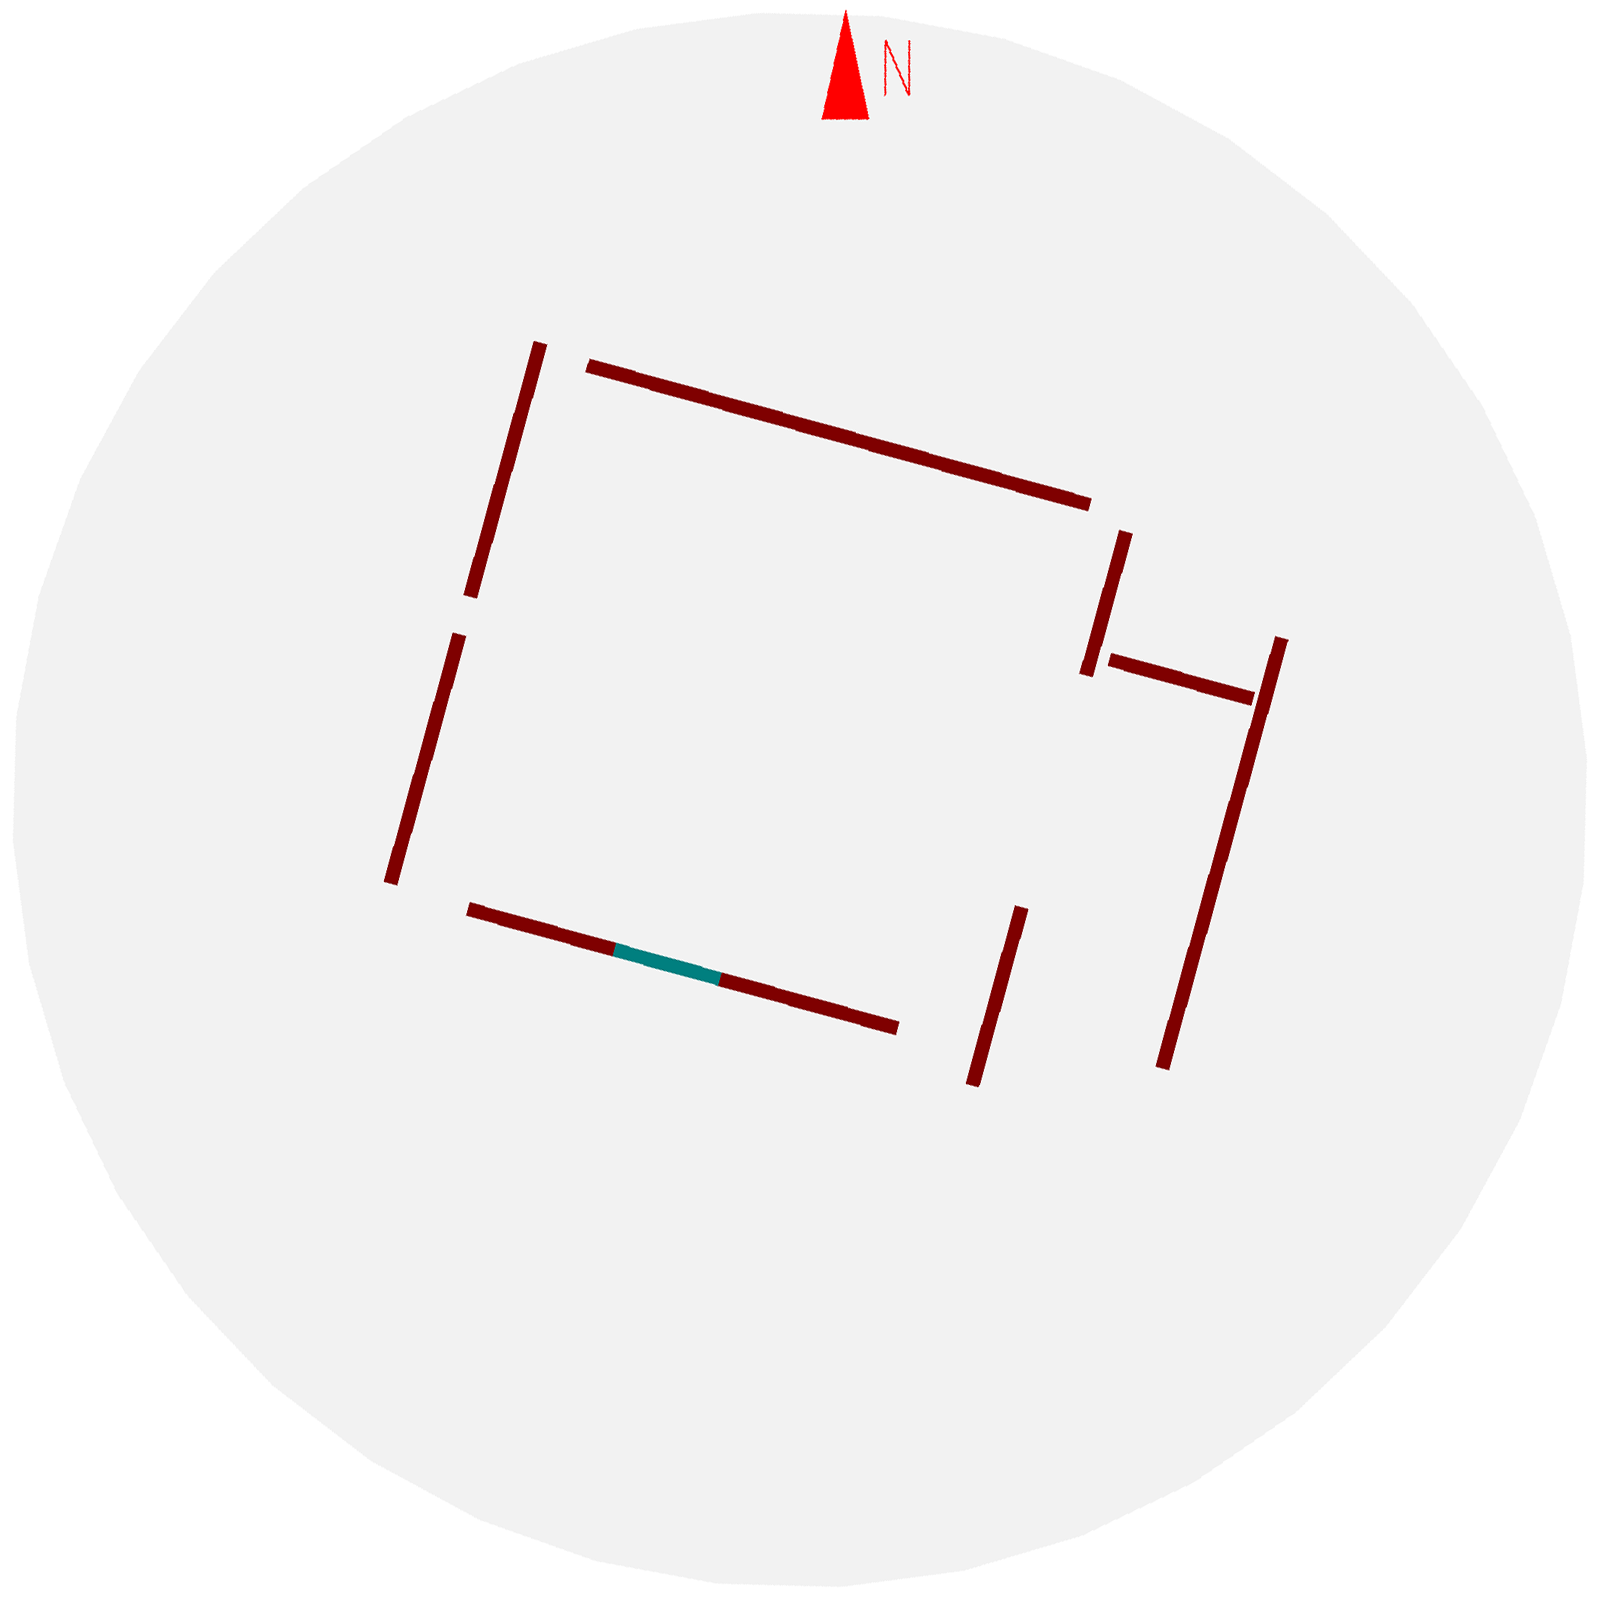
\includegraphics[width=0.95in]{../gi2012_userstudy/images/section2/2_2D_walls_rotate} %A2
  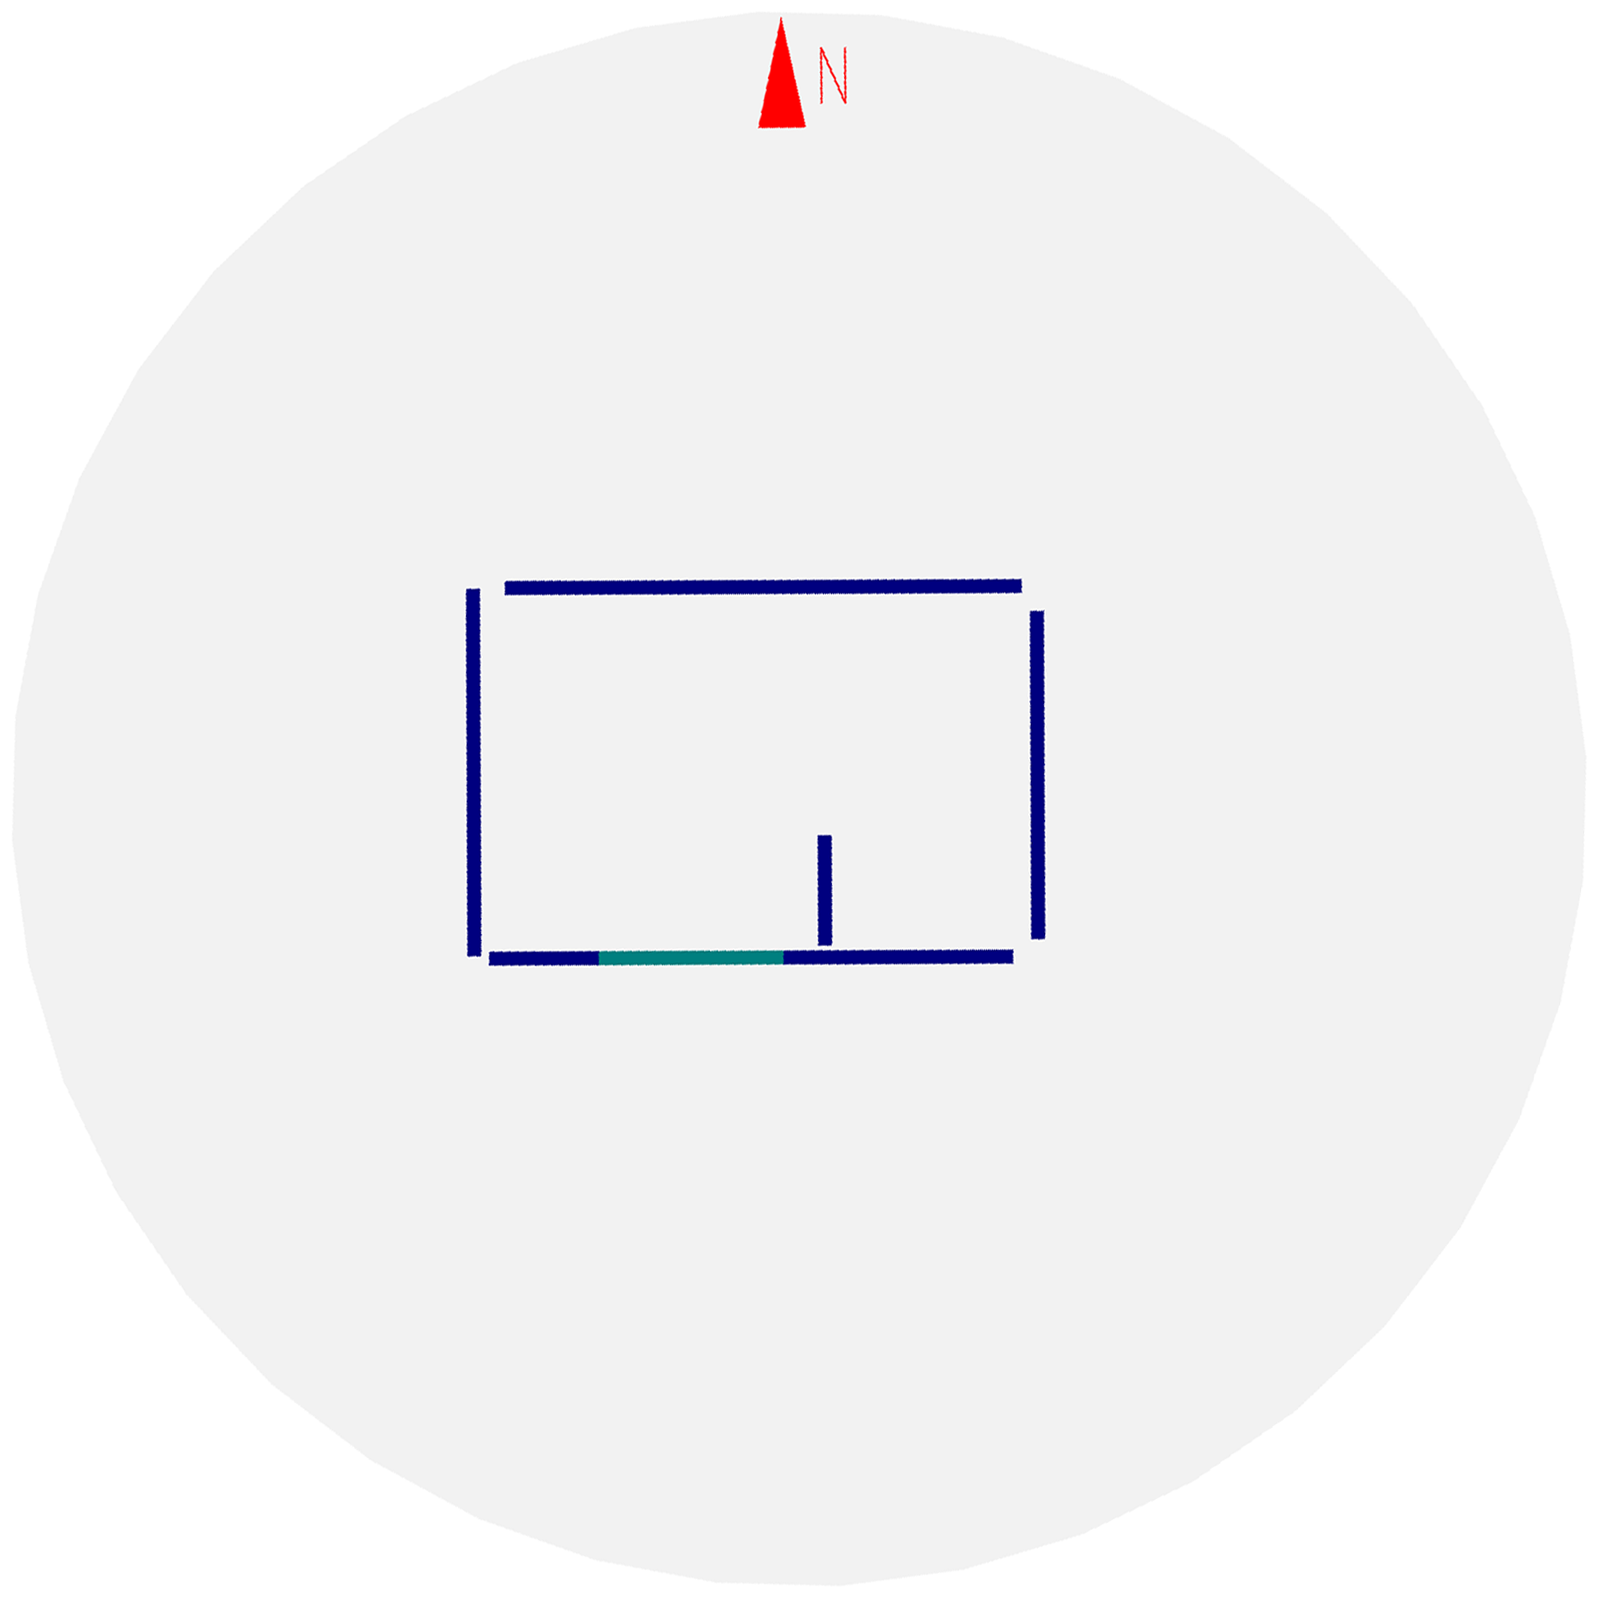
\includegraphics[width=0.95in]{../gi2012_userstudy/images/section2/6_2D_walls_rotate}  %A4
  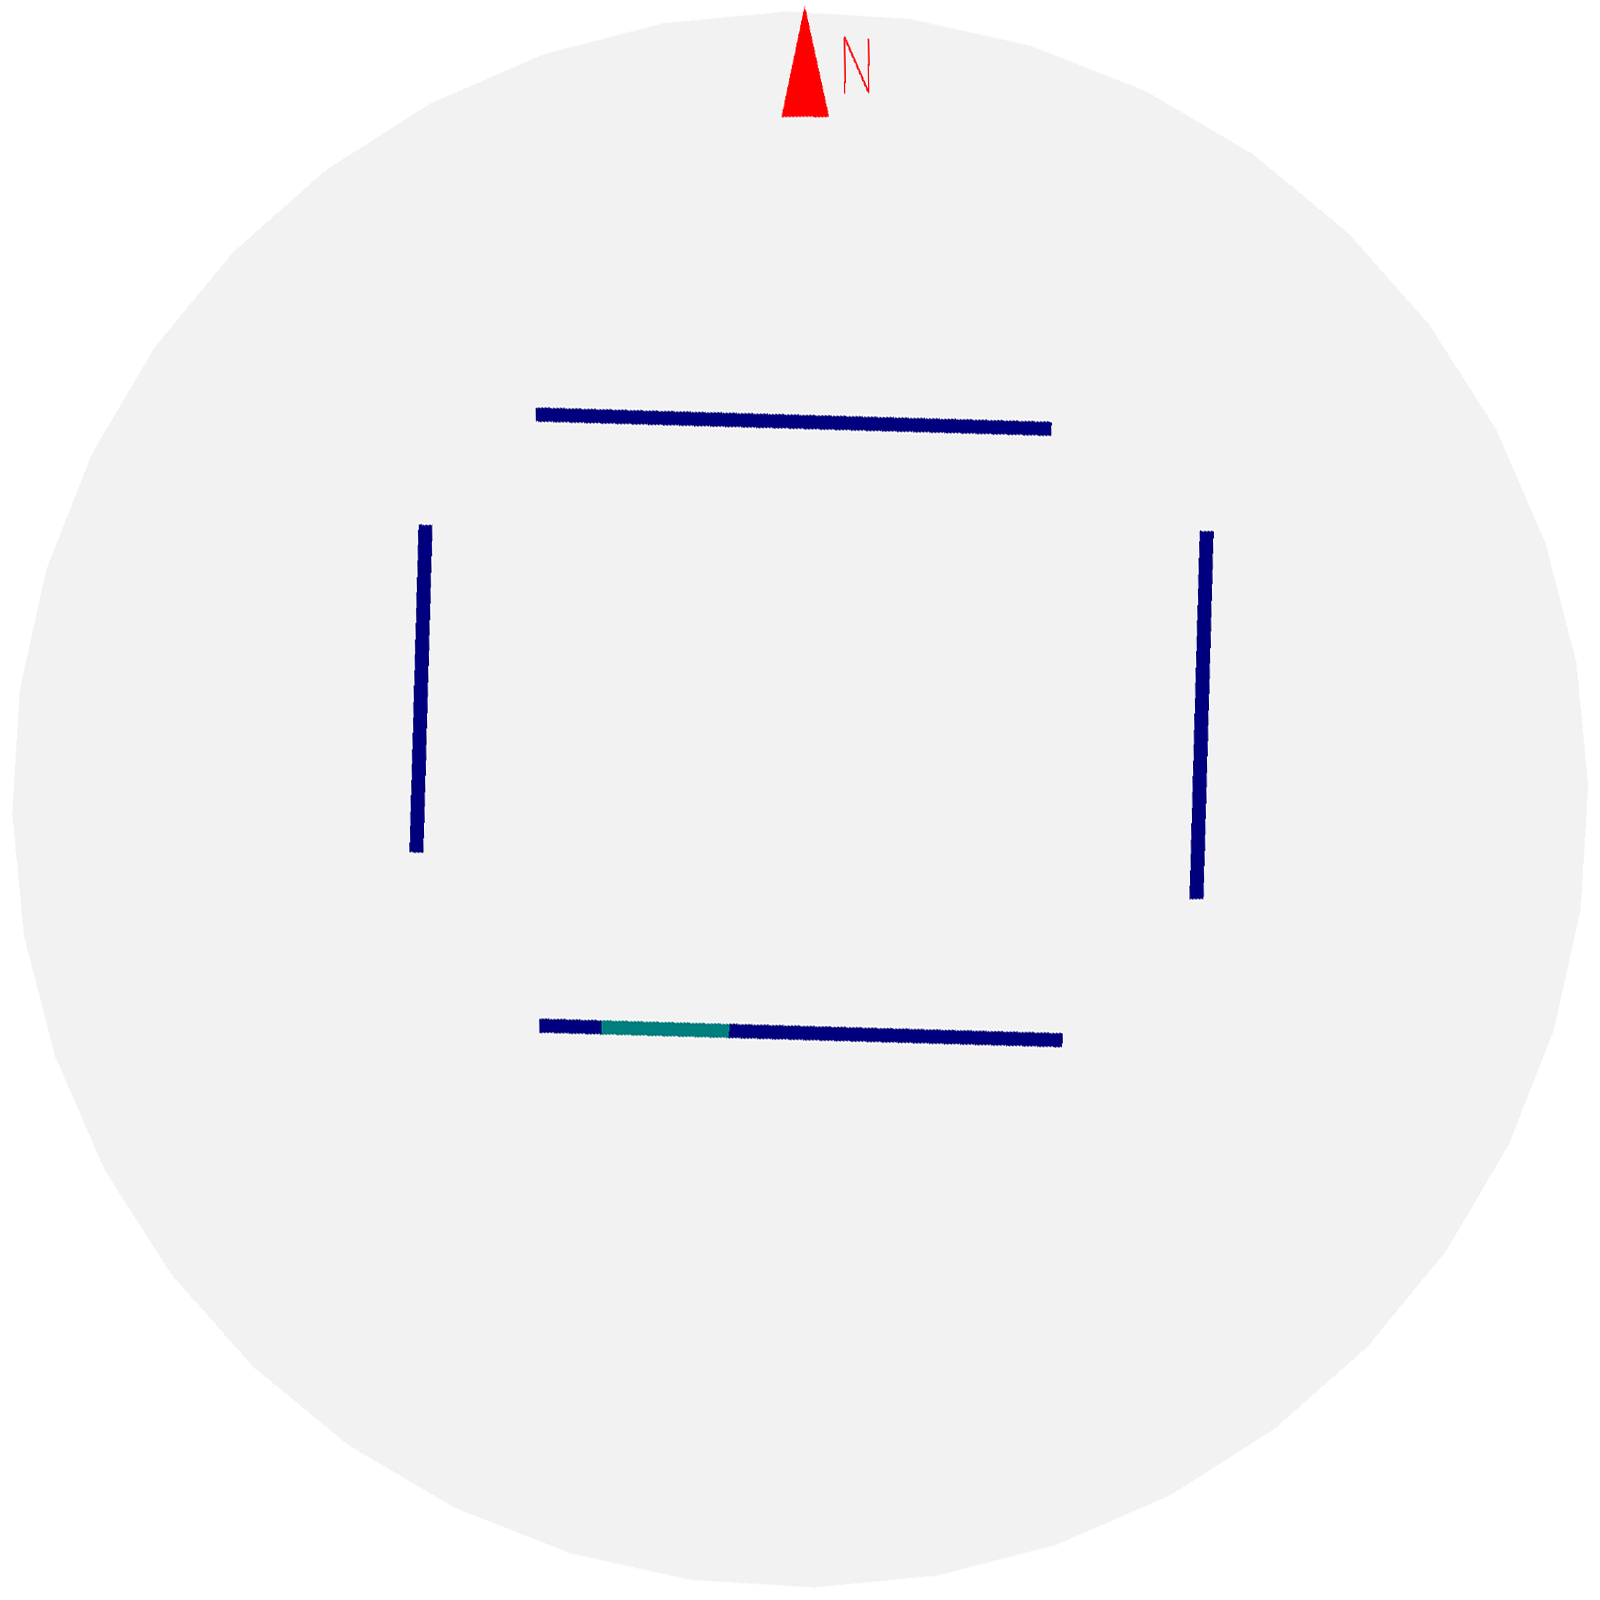
\includegraphics[width=0.95in]{../gi2012_userstudy/images/section2/7_2D_walls_rotate} %A5
  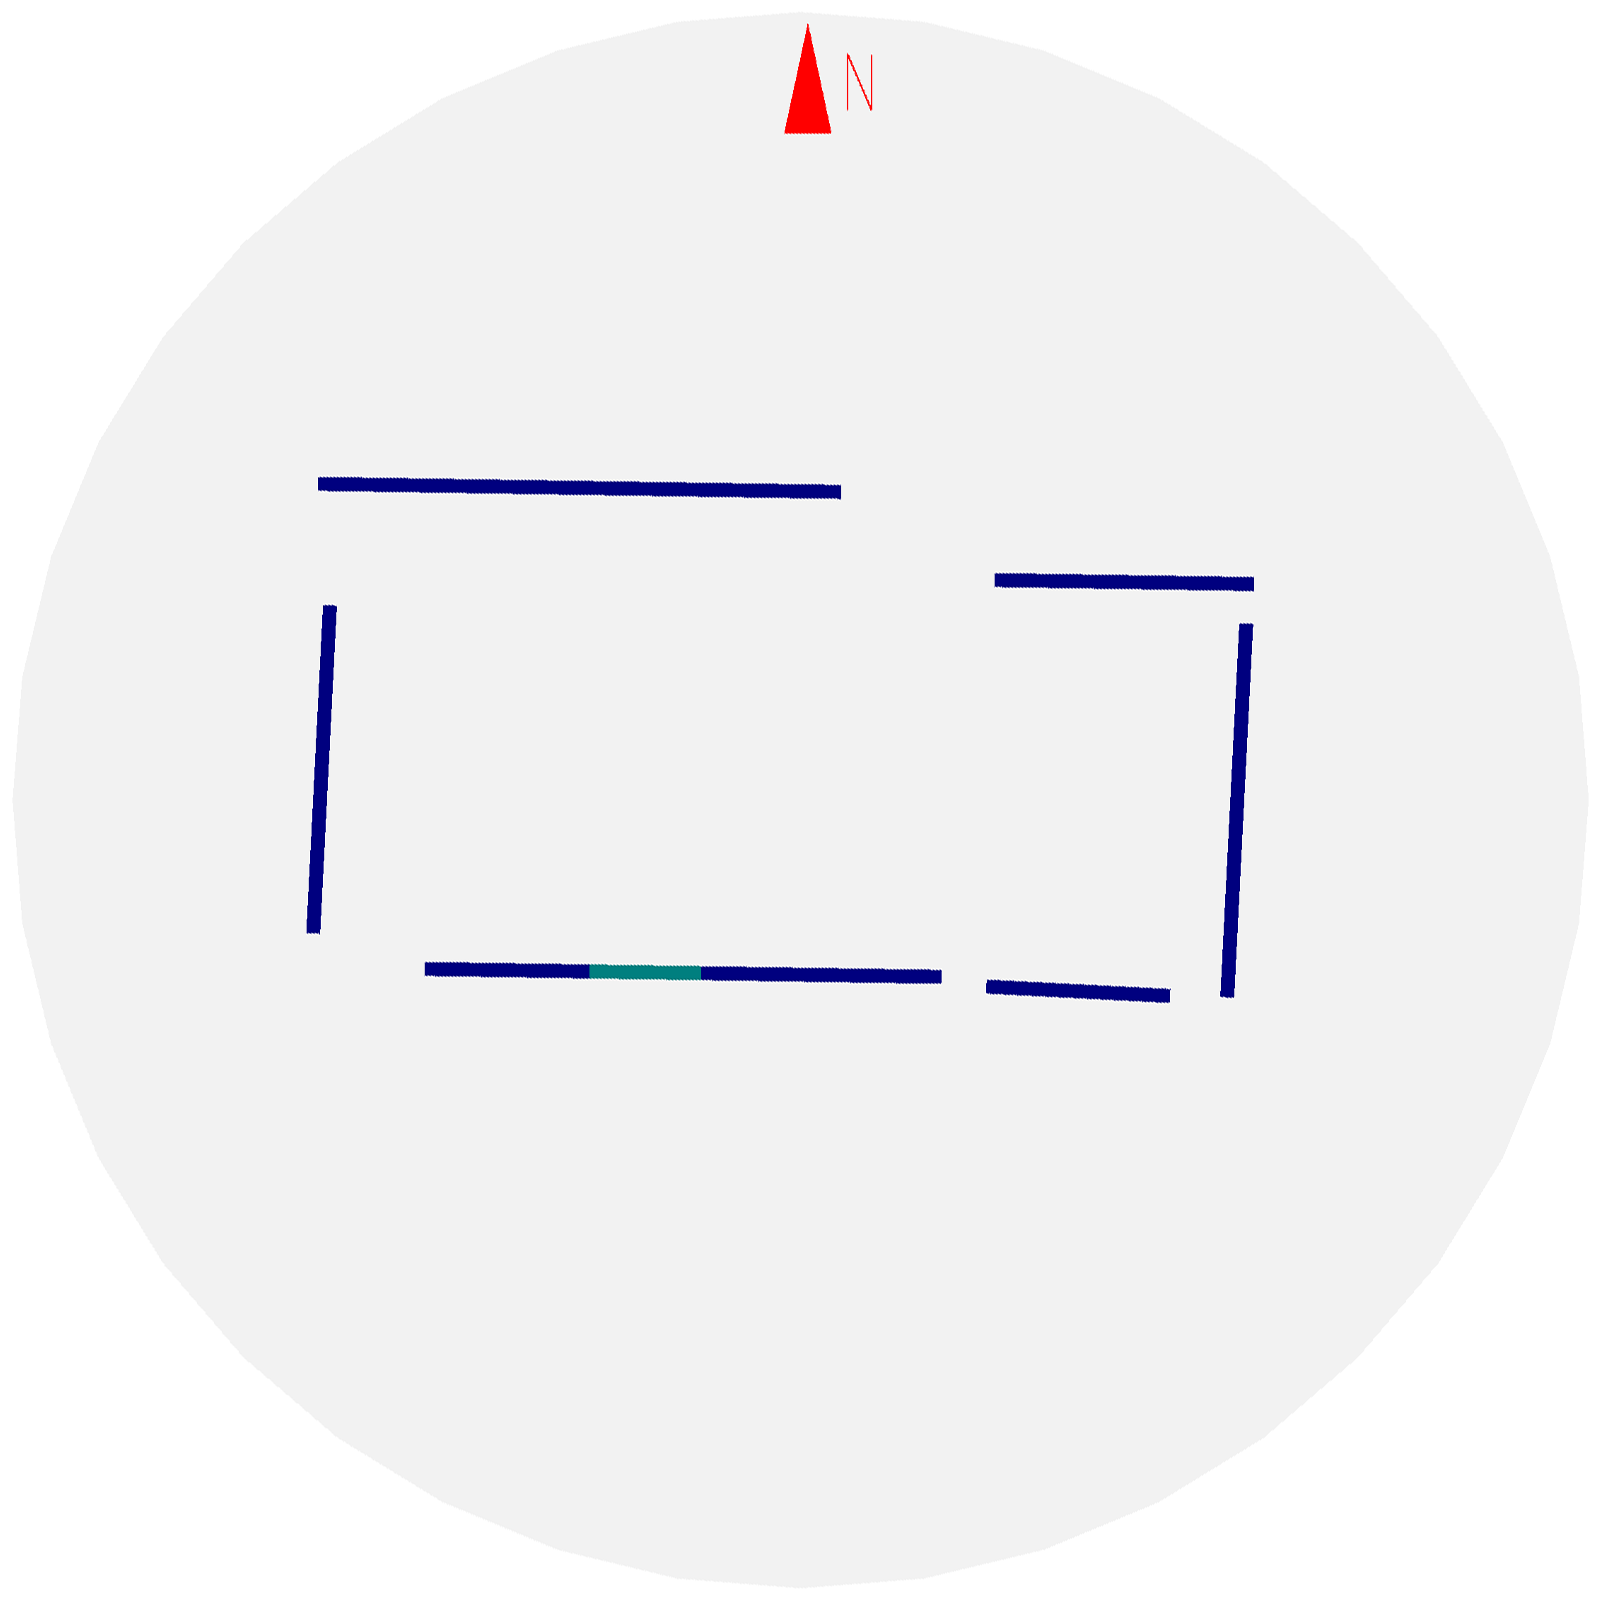
\includegraphics[width=0.95in]{../gi2012_userstudy/images/section2/8_2D_walls_rotate}\\ %A6
  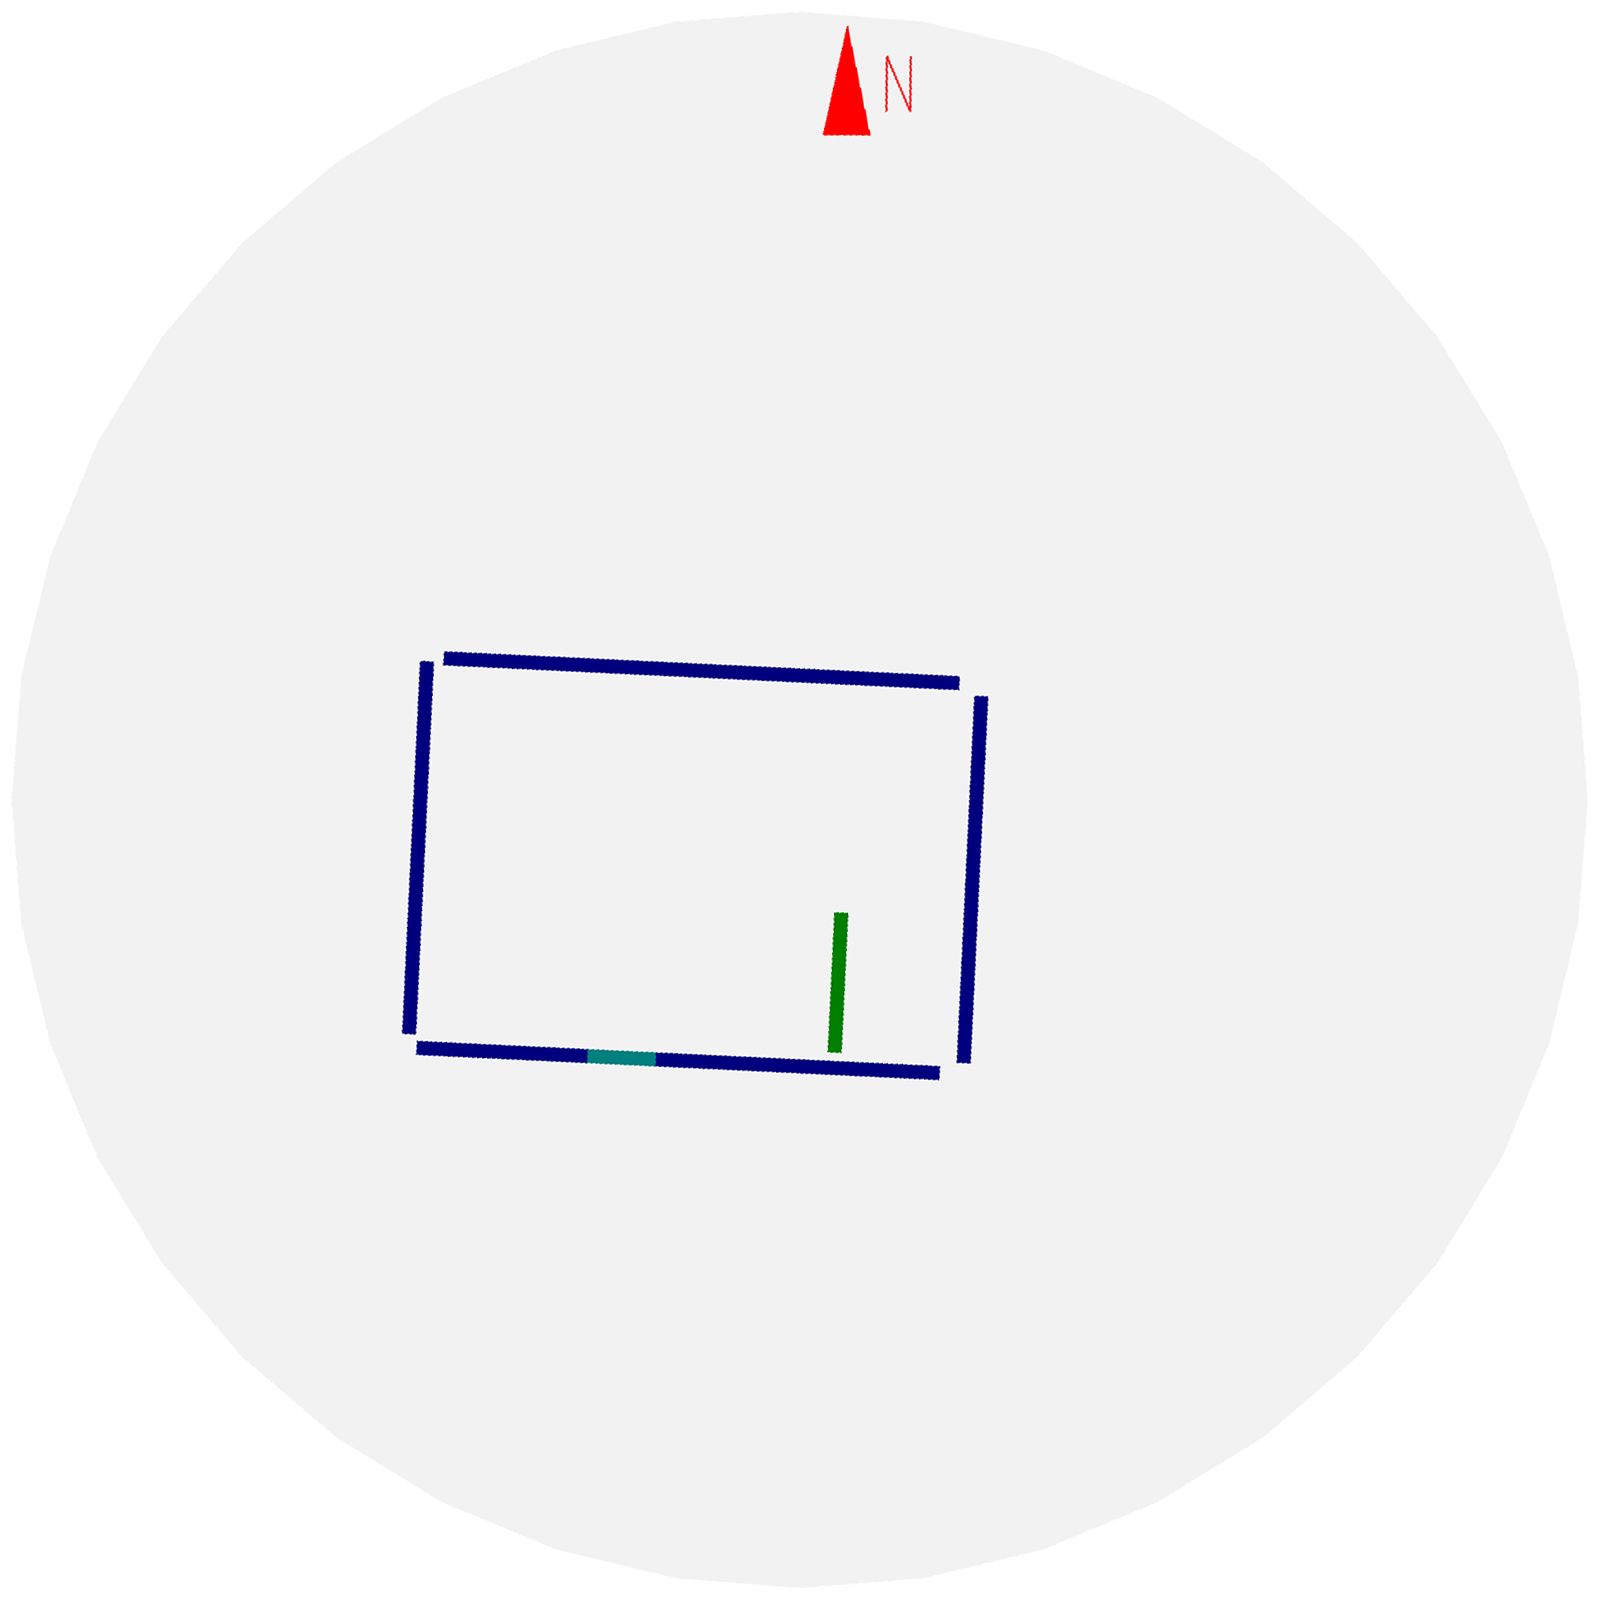
\includegraphics[width=0.95in]{../gi2012_userstudy/images/section2/3_2D_walls_rotate} %N2
  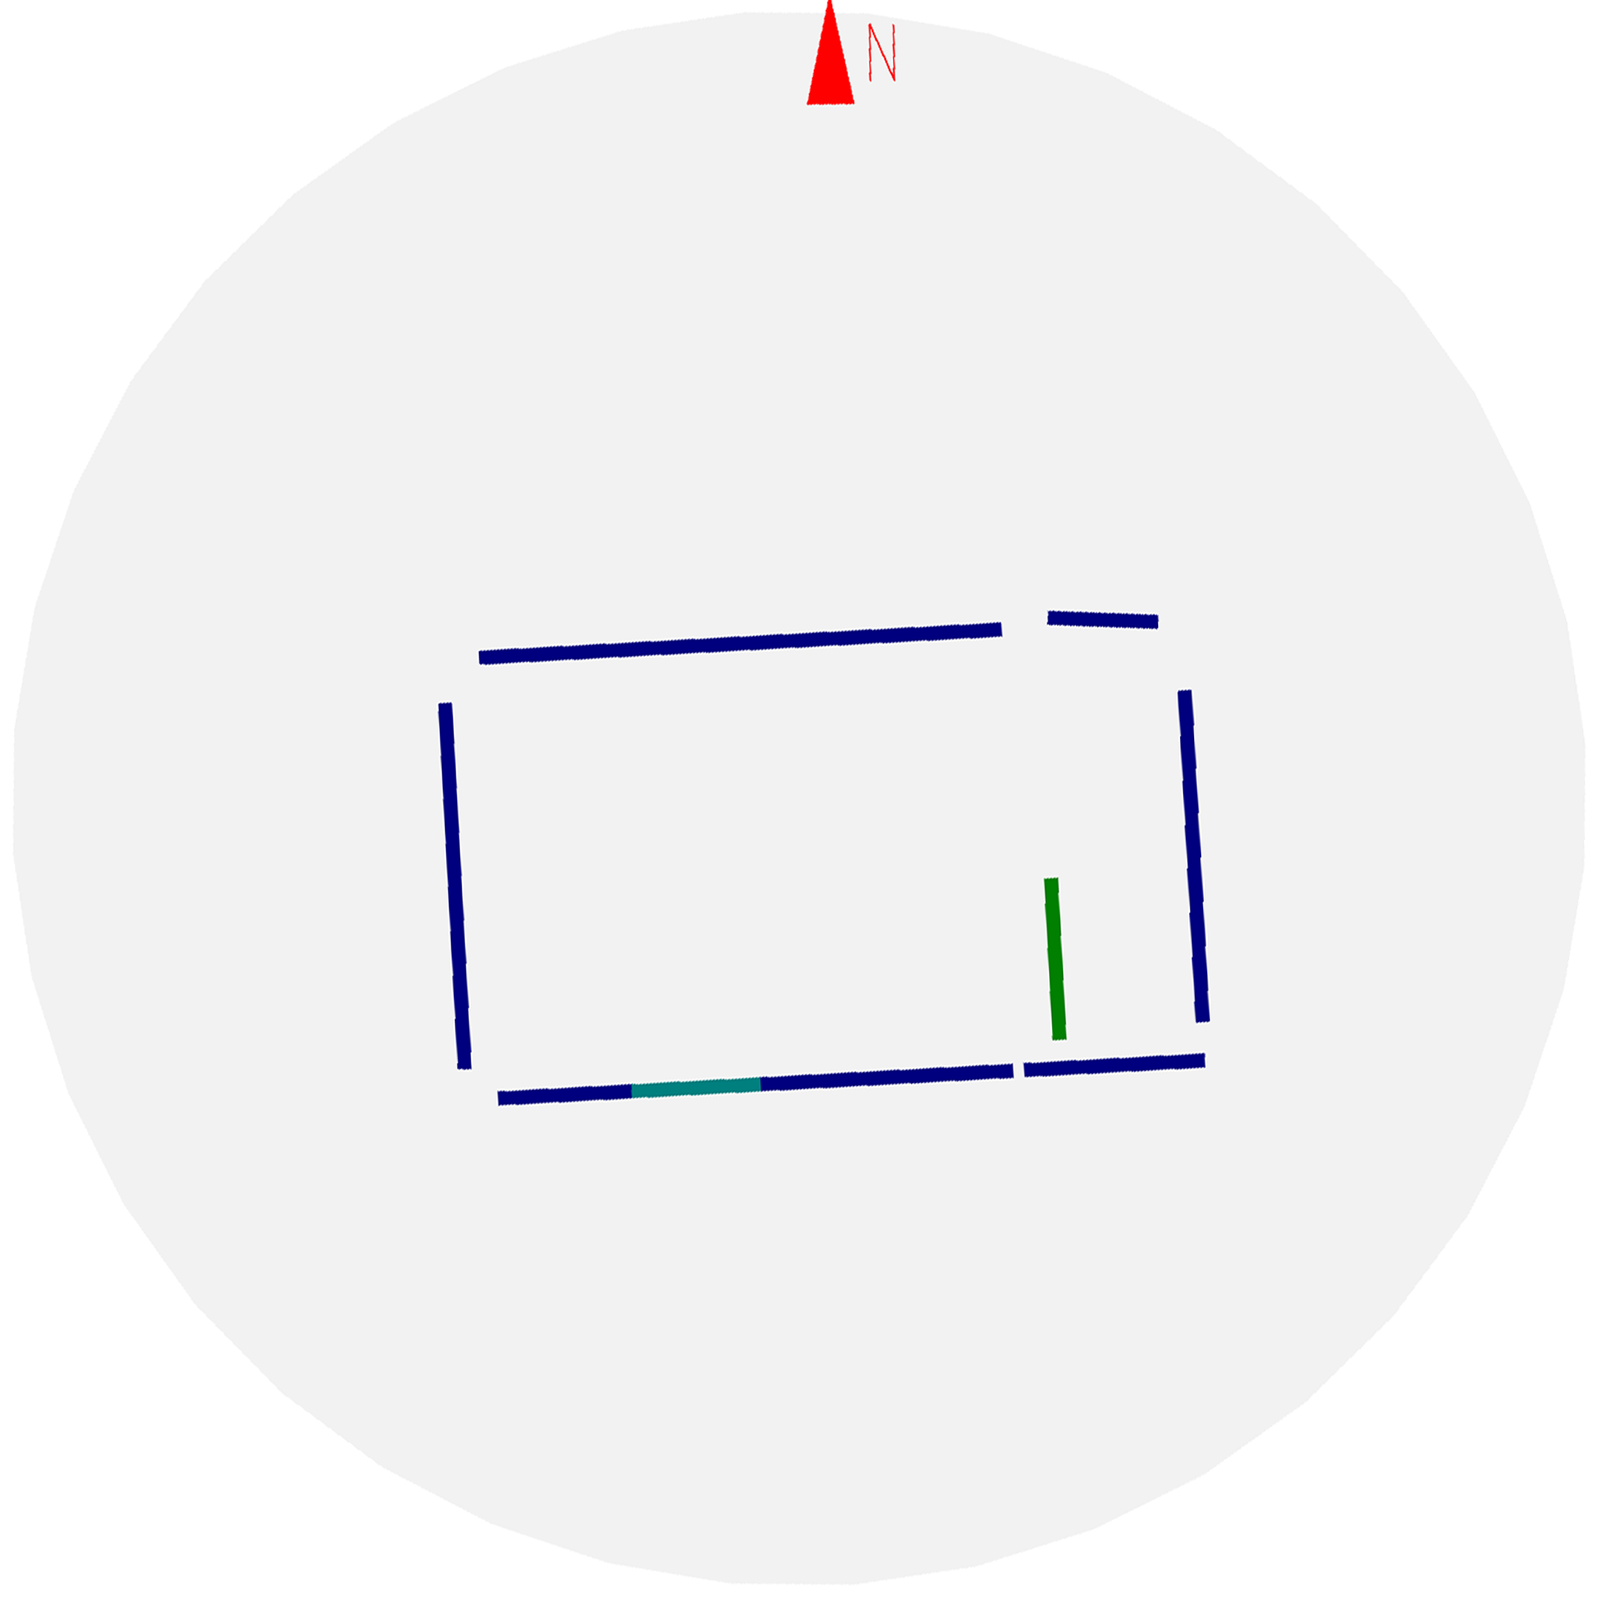
\includegraphics[width=0.95in]{../gi2012_userstudy/images/section2/5_2D_walls_rotate} %N4
  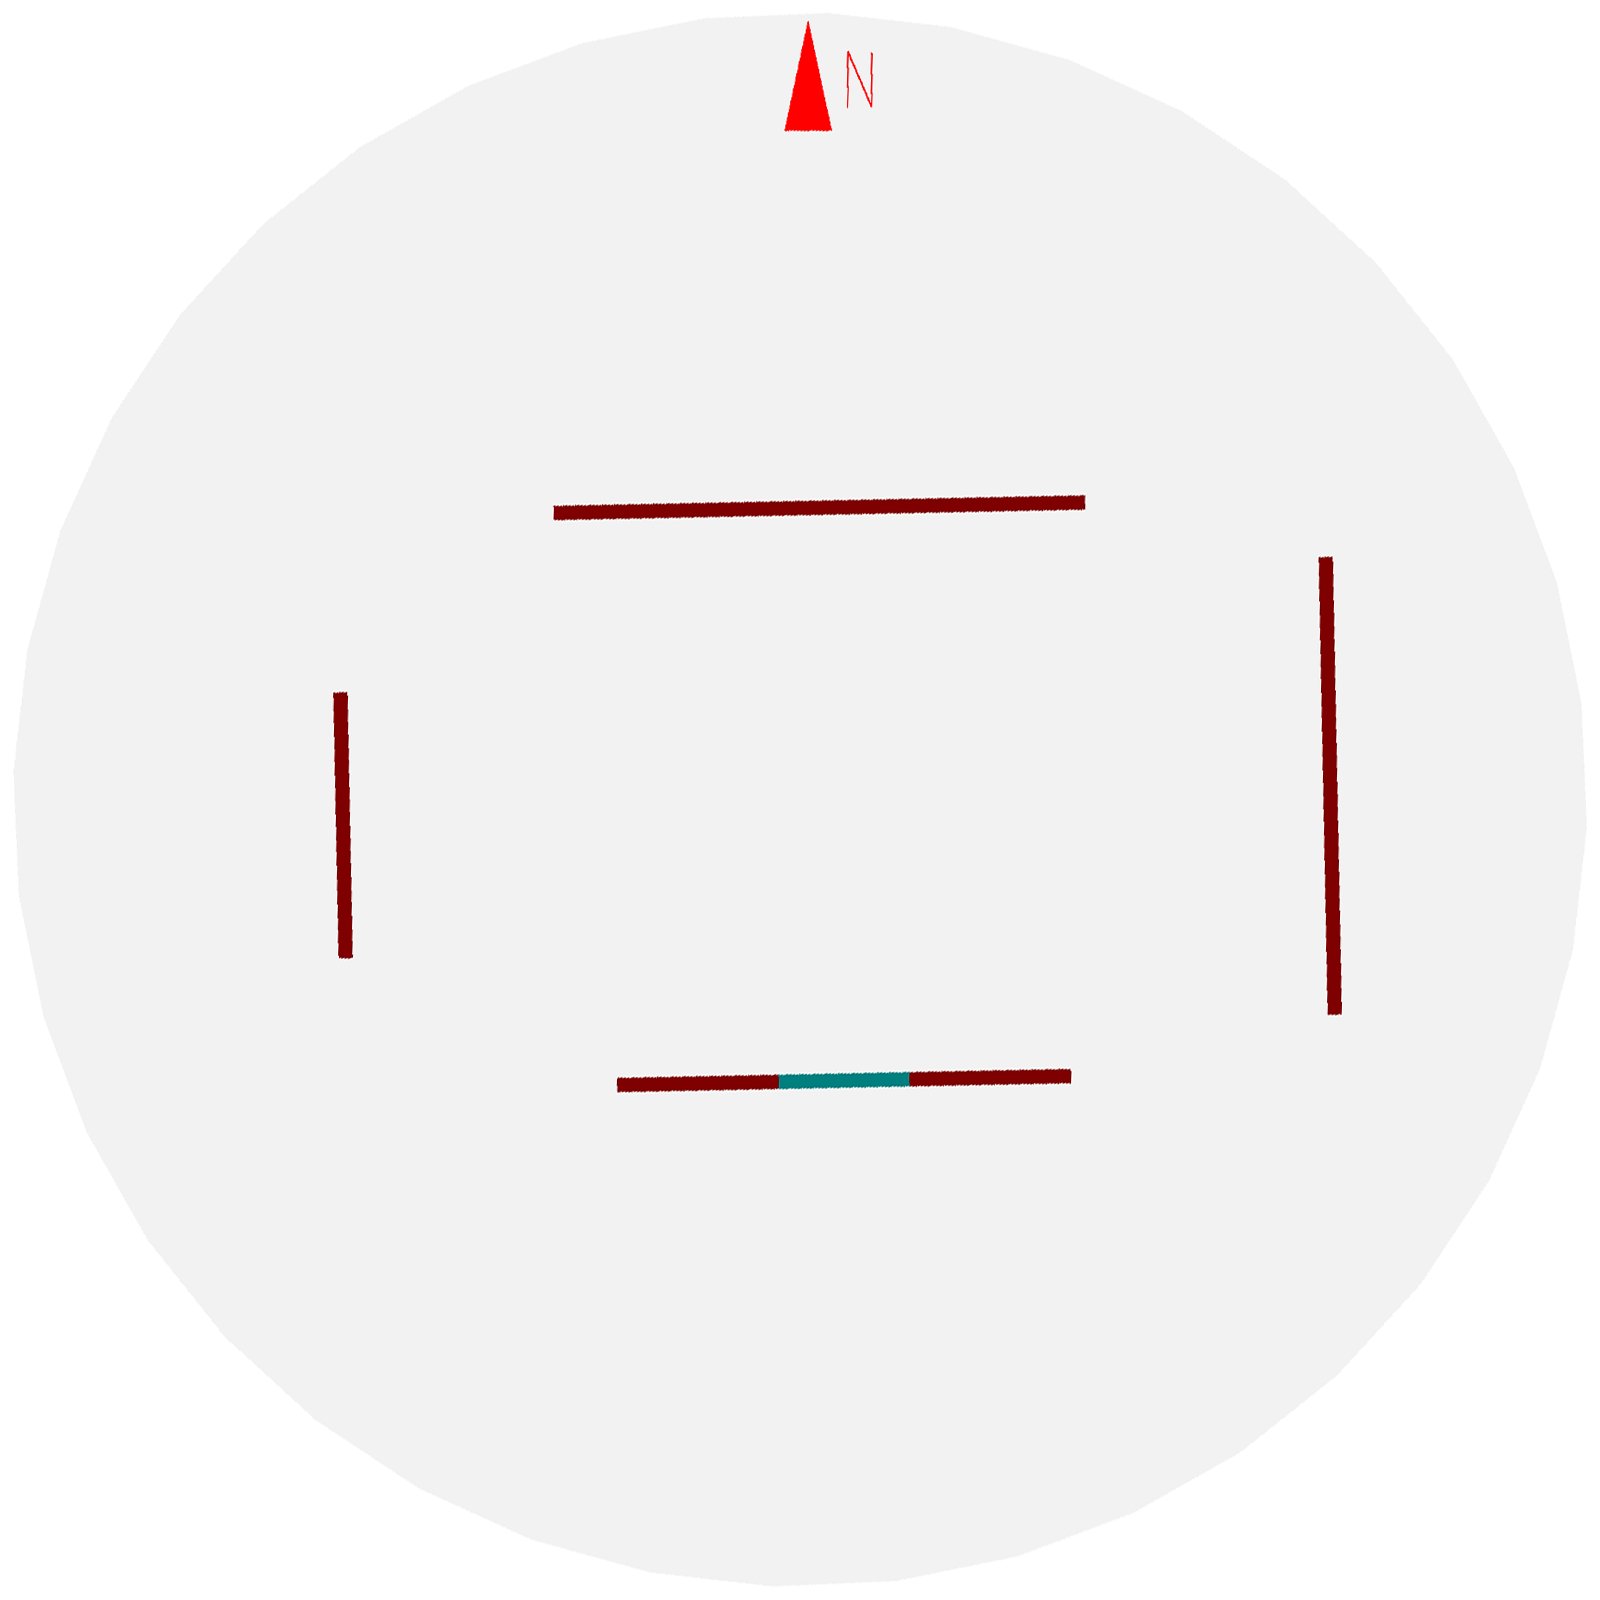
\includegraphics[width=0.95in]{../gi2012_userstudy/images/section2/9_2D_walls_rotate} %N5
  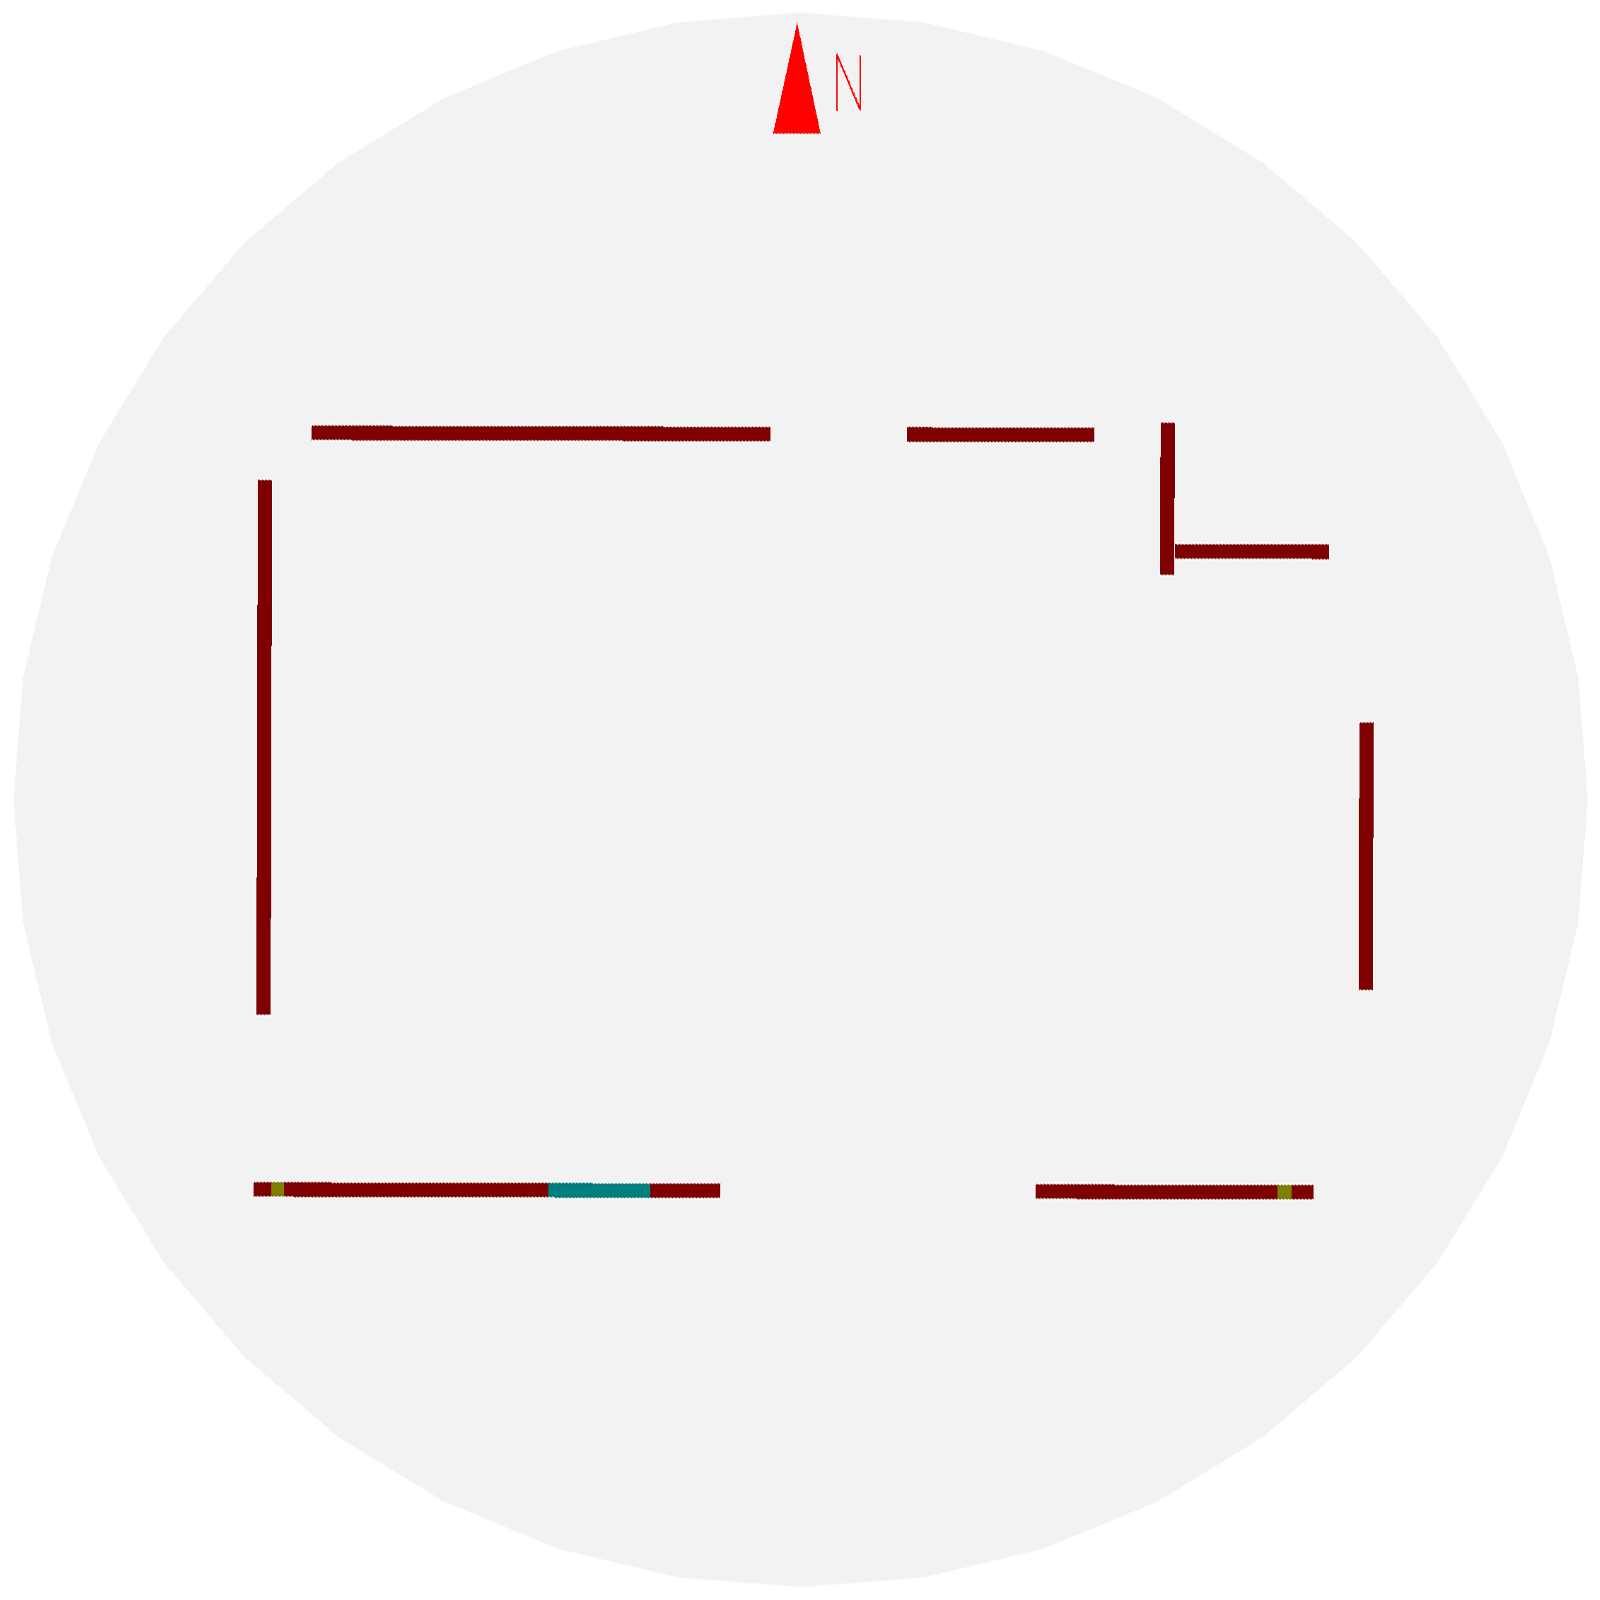
\includegraphics[width=0.95in]{../gi2012_userstudy/images/section2/10_2D_walls_rotate} %N6
  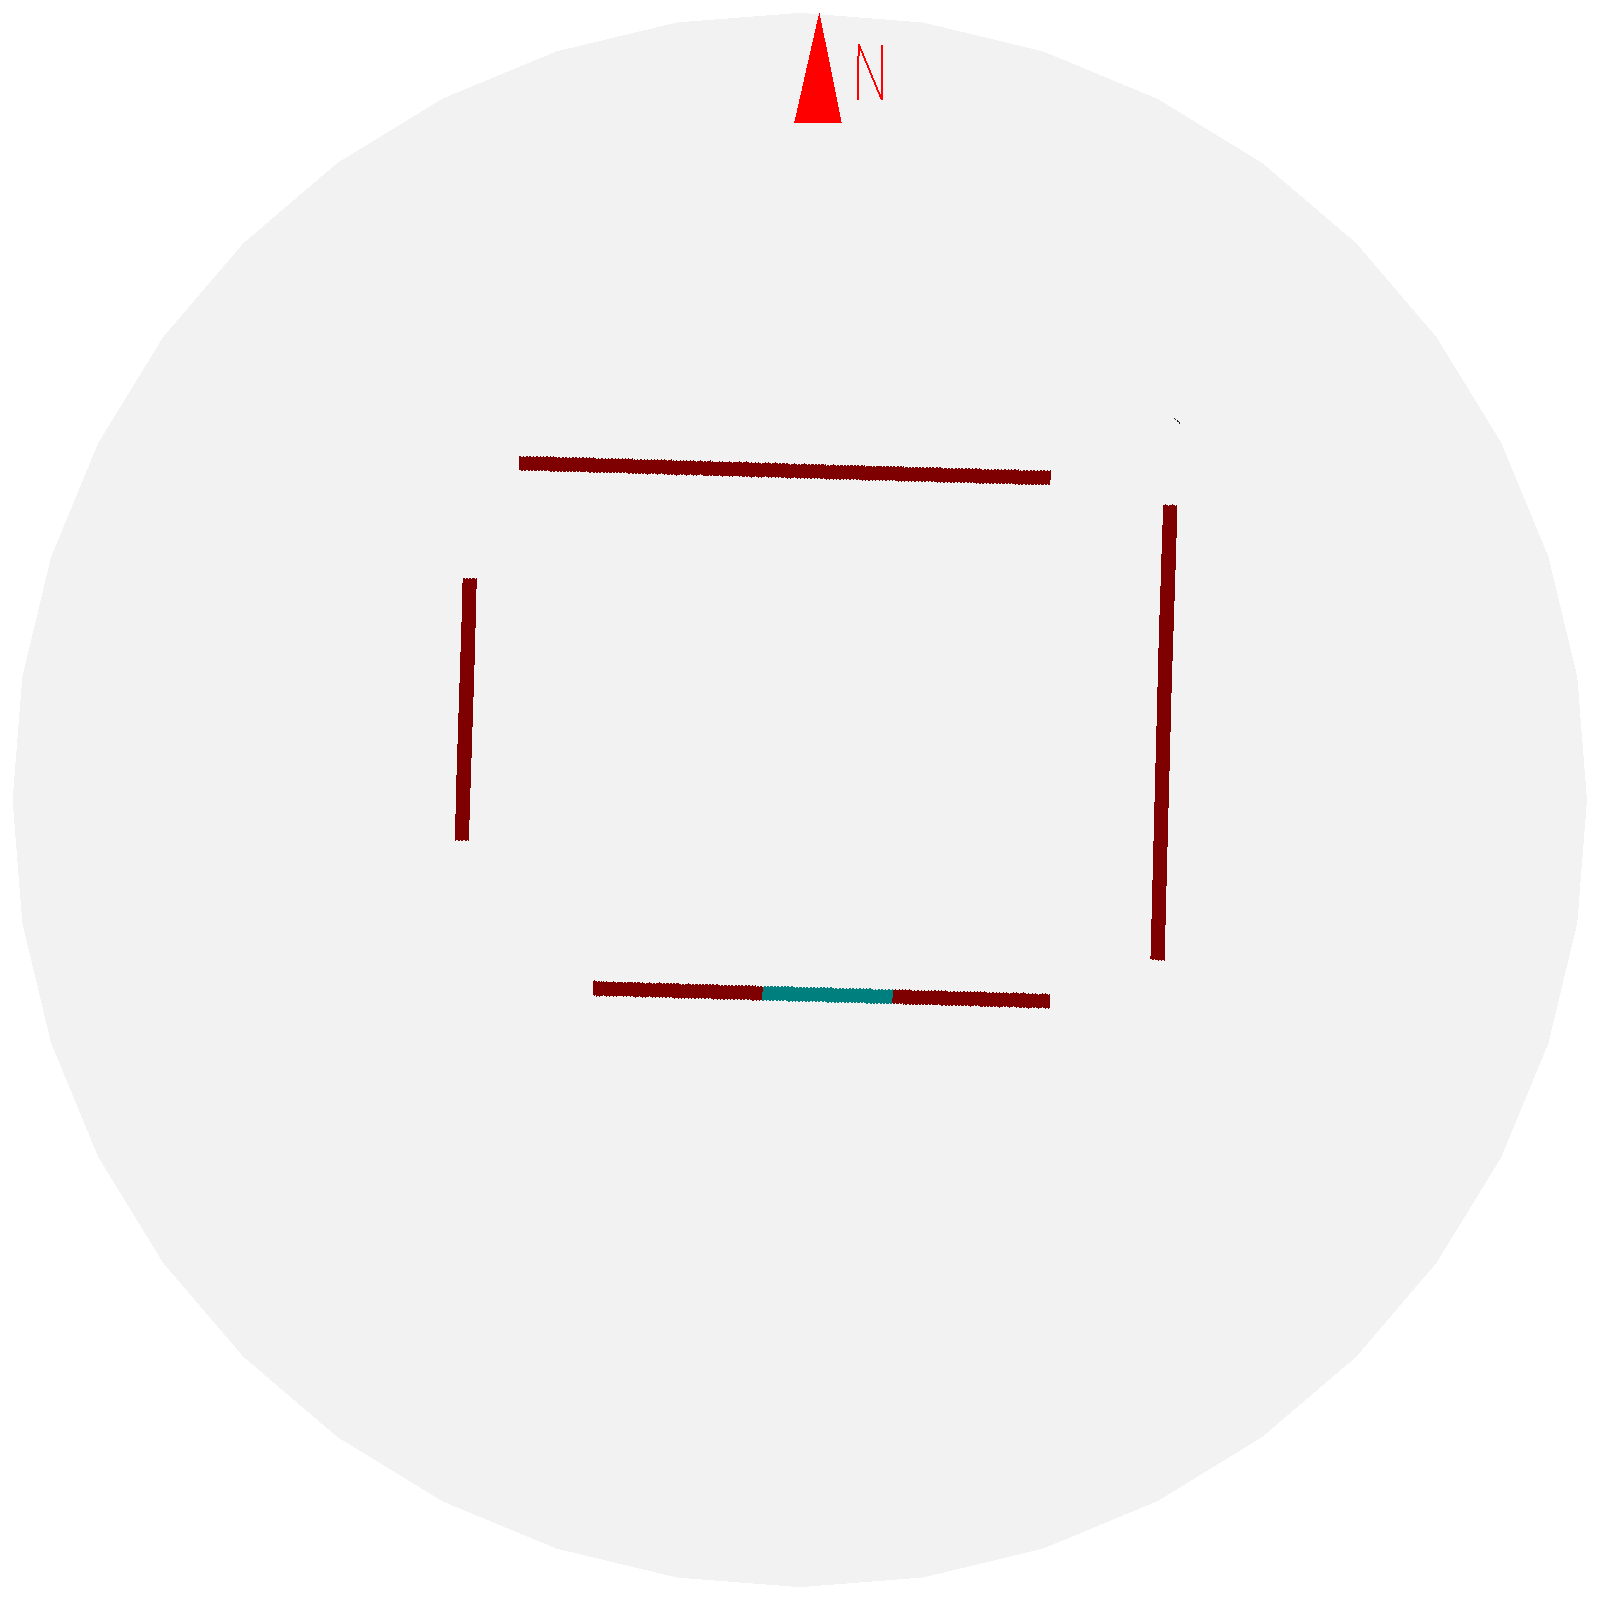
\includegraphics[width=0.95in]{../gi2012_userstudy/images/section2/11_2D_walls_rotate} %N7
\end{minipage}
\vspace{-1.12in}
\\
\begin{minipage}{1.92in}~\end{minipage}
\begin{minipage}{0.95in}{\bf A1}\end{minipage}
\begin{minipage}{0.95in}{\bf A2}\end{minipage}
\begin{minipage}{0.95in}{\bf A4}\end{minipage}
\begin{minipage}{0.95in}{\bf A5}\end{minipage}
\begin{minipage}{0.95in}{\bf A6}\end{minipage}
\vspace{0.78in}
\\
\begin{minipage}{1.92in}{\bf ~N1}\end{minipage}
\begin{minipage}{0.95in}{\bf N2}\end{minipage}
\begin{minipage}{0.95in}{\bf N4}\end{minipage}
\begin{minipage}{0.95in}{\bf N5}\end{minipage}
\begin{minipage}{0.95in}{\bf N6}\end{minipage}
\begin{minipage}{0.95in}{\bf N7}\end{minipage}\vspace{-0.08in}%\\
\end{center}
  \caption{
  \label{figure:original_designs}
A photograph of the physical geometry of the original office space
constructed by one of the participants for Part 2 of the study and 2D
diagrams of the geometry constructed by the other participants. 
% Note
%the variety of model complexity and scale that users create to
%represent the same space.  The red walls are 10 inches tall and the
%blue walls are 8 inches tall.  Global illumination renderings of these
%geometries are shown in
%Figure~\ref{figure:renderingsOfOriginalGeometry}.
}
\end{figure*}

